\section{PVToPV\_\-swa Class Reference}
\label{classPVToPV__swa}\index{PVToPV\_\-swa@{PVToPV\_\-swa}}
{\tt \#include $<$pvtopv\_\-swa.h$>$}

Collaboration diagram for PVToPV\_\-swa:\nopagebreak
\begin{figure}[H]
\begin{center}
\leavevmode
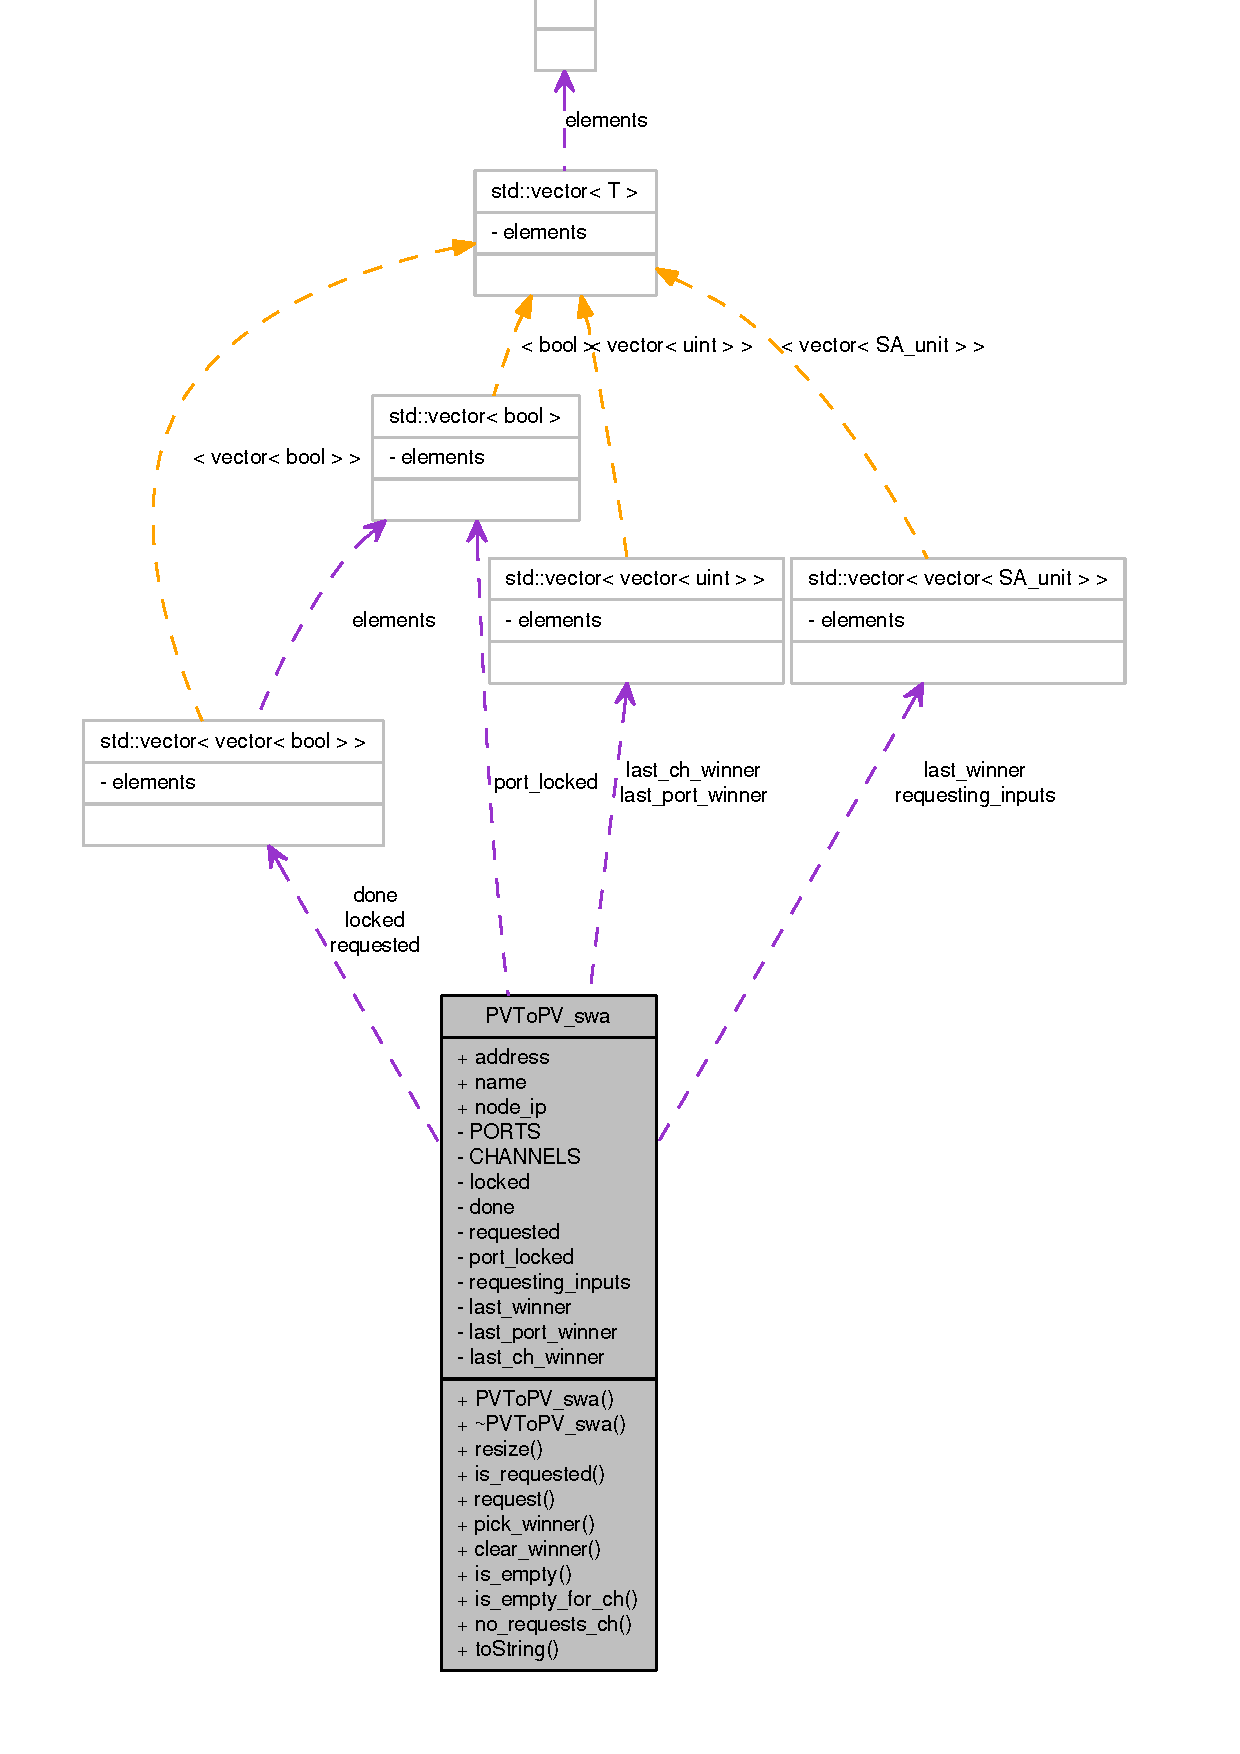
\includegraphics[width=400pt]{classPVToPV__swa__coll__graph}
\end{center}
\end{figure}
\subsection*{Public Member Functions}
\begin{CompactItemize}
\item 
{\bf PVToPV\_\-swa} ()
\item 
{\bf $\sim$PVToPV\_\-swa} ()
\item 
void {\bf resize} ({\bf uint} p, {\bf uint} c)
\item 
bool {\bf is\_\-requested} ({\bf uint} inp, {\bf uint} inch, {\bf uint} p, {\bf uint} c)
\item 
void {\bf request} ({\bf uint} p, {\bf uint} c, {\bf uint} inp, {\bf uint} inch)
\item 
{\bf SA\_\-unit} {\bf pick\_\-winner} ({\bf uint} p, {\bf uint} c)
\item 
void {\bf clear\_\-winner} ({\bf uint} p, {\bf uint} c, {\bf uint} ip, {\bf uint} ic)
\item 
bool {\bf is\_\-empty} ()
\item 
bool {\bf is\_\-empty\_\-for\_\-ch} ({\bf uint} ch)
\item 
{\bf uint} {\bf no\_\-requests\_\-ch} ({\bf uint} ch)
\item 
string {\bf toString} () const 
\end{CompactItemize}
\subsection*{Public Attributes}
\begin{CompactItemize}
\item 
{\bf uint} {\bf address}
\item 
{\bf uint} {\bf name}
\item 
{\bf uint} {\bf node\_\-ip}
\end{CompactItemize}
\subsection*{Private Attributes}
\begin{CompactItemize}
\item 
{\bf uint} {\bf PORTS}
\item 
{\bf uint} {\bf CHANNELS}
\item 
vector$<$ vector$<$ bool $>$ $>$ {\bf locked}
\item 
vector$<$ vector$<$ bool $>$ $>$ {\bf done}
\item 
vector$<$ vector$<$ bool $>$ $>$ {\bf requested}
\item 
vector$<$ bool $>$ {\bf port\_\-locked}
\item 
vector$<$ vector$<$ {\bf SA\_\-unit} $>$ $>$ {\bf requesting\_\-inputs}
\item 
vector$<$ vector$<$ {\bf SA\_\-unit} $>$ $>$ {\bf last\_\-winner}
\item 
vector$<$ vector$<$ {\bf uint} $>$ $>$ {\bf last\_\-port\_\-winner}
\item 
vector$<$ vector$<$ {\bf uint} $>$ $>$ {\bf last\_\-ch\_\-winner}
\end{CompactItemize}


\subsection{Detailed Description}


Definition at line 27 of file pvtopv\_\-swa.h.

\subsection{Constructor \& Destructor Documentation}
\index{PVToPV\_\-swa@{PVToPV\_\-swa}!PVToPV\_\-swa@{PVToPV\_\-swa}}
\index{PVToPV\_\-swa@{PVToPV\_\-swa}!PVToPV_swa@{PVToPV\_\-swa}}
\subsubsection[{PVToPV\_\-swa}]{\setlength{\rightskip}{0pt plus 5cm}PVToPV\_\-swa::PVToPV\_\-swa ()}\label{classPVToPV__swa_e61260956d80cbb85fbc88cc4405cbb1}




Definition at line 24 of file pvtopv\_\-swa.cc.\index{PVToPV\_\-swa@{PVToPV\_\-swa}!$\sim$PVToPV\_\-swa@{$\sim$PVToPV\_\-swa}}
\index{$\sim$PVToPV\_\-swa@{$\sim$PVToPV\_\-swa}!PVToPV_swa@{PVToPV\_\-swa}}
\subsubsection[{$\sim$PVToPV\_\-swa}]{\setlength{\rightskip}{0pt plus 5cm}PVToPV\_\-swa::$\sim$PVToPV\_\-swa ()}\label{classPVToPV__swa_cf2004091e12ac26b24e31124337e989}




Definition at line 29 of file pvtopv\_\-swa.cc.

\subsection{Member Function Documentation}
\index{PVToPV\_\-swa@{PVToPV\_\-swa}!clear\_\-winner@{clear\_\-winner}}
\index{clear\_\-winner@{clear\_\-winner}!PVToPV_swa@{PVToPV\_\-swa}}
\subsubsection[{clear\_\-winner}]{\setlength{\rightskip}{0pt plus 5cm}void PVToPV\_\-swa::clear\_\-winner ({\bf uint} {\em p}, \/  {\bf uint} {\em c}, \/  {\bf uint} {\em ip}, \/  {\bf uint} {\em ic})}\label{classPVToPV__swa_16391cc301306acef66eff1ab847c7ca}




Definition at line 150 of file pvtopv\_\-swa.cc.

References CHANNELS, done, locked, and requested.\index{PVToPV\_\-swa@{PVToPV\_\-swa}!is\_\-empty@{is\_\-empty}}
\index{is\_\-empty@{is\_\-empty}!PVToPV_swa@{PVToPV\_\-swa}}
\subsubsection[{is\_\-empty}]{\setlength{\rightskip}{0pt plus 5cm}bool PVToPV\_\-swa::is\_\-empty (void)}\label{classPVToPV__swa_2c5f9c5a78aa05ab166b58d04738081d}




Definition at line 160 of file pvtopv\_\-swa.cc.

References CHANNELS, PORTS, and requested.\index{PVToPV\_\-swa@{PVToPV\_\-swa}!is\_\-empty\_\-for\_\-ch@{is\_\-empty\_\-for\_\-ch}}
\index{is\_\-empty\_\-for\_\-ch@{is\_\-empty\_\-for\_\-ch}!PVToPV_swa@{PVToPV\_\-swa}}
\subsubsection[{is\_\-empty\_\-for\_\-ch}]{\setlength{\rightskip}{0pt plus 5cm}bool PVToPV\_\-swa::is\_\-empty\_\-for\_\-ch ({\bf uint} {\em ch})}\label{classPVToPV__swa_131c0ee2c54b76f6c10858889104edb4}




Definition at line 174 of file pvtopv\_\-swa.cc.

References requested.\index{PVToPV\_\-swa@{PVToPV\_\-swa}!is\_\-requested@{is\_\-requested}}
\index{is\_\-requested@{is\_\-requested}!PVToPV_swa@{PVToPV\_\-swa}}
\subsubsection[{is\_\-requested}]{\setlength{\rightskip}{0pt plus 5cm}bool PVToPV\_\-swa::is\_\-requested ({\bf uint} {\em inp}, \/  {\bf uint} {\em inch}, \/  {\bf uint} {\em p}, \/  {\bf uint} {\em c})}\label{classPVToPV__swa_bc1410b2178d02ce2bacba66707e1b1e}




Definition at line 82 of file pvtopv\_\-swa.cc.

References locked.\index{PVToPV\_\-swa@{PVToPV\_\-swa}!no\_\-requests\_\-ch@{no\_\-requests\_\-ch}}
\index{no\_\-requests\_\-ch@{no\_\-requests\_\-ch}!PVToPV_swa@{PVToPV\_\-swa}}
\subsubsection[{no\_\-requests\_\-ch}]{\setlength{\rightskip}{0pt plus 5cm}{\bf uint} PVToPV\_\-swa::no\_\-requests\_\-ch ({\bf uint} {\em ch})}\label{classPVToPV__swa_31bf97288ff71191f3fc7210d29976a9}




Definition at line 183 of file pvtopv\_\-swa.cc.

References requested.\index{PVToPV\_\-swa@{PVToPV\_\-swa}!pick\_\-winner@{pick\_\-winner}}
\index{pick\_\-winner@{pick\_\-winner}!PVToPV_swa@{PVToPV\_\-swa}}
\subsubsection[{pick\_\-winner}]{\setlength{\rightskip}{0pt plus 5cm}{\bf SA\_\-unit} PVToPV\_\-swa::pick\_\-winner ({\bf uint} {\em p}, \/  {\bf uint} {\em c})}\label{classPVToPV__swa_957d1cb1cd6ffa264749dd89e2ae1cd1}




Definition at line 100 of file pvtopv\_\-swa.cc.

References CHANNELS, done, last\_\-port\_\-winner, last\_\-winner, locked, PORTS, requested, and requesting\_\-inputs.\index{PVToPV\_\-swa@{PVToPV\_\-swa}!request@{request}}
\index{request@{request}!PVToPV_swa@{PVToPV\_\-swa}}
\subsubsection[{request}]{\setlength{\rightskip}{0pt plus 5cm}void PVToPV\_\-swa::request ({\bf uint} {\em p}, \/  {\bf uint} {\em c}, \/  {\bf uint} {\em inp}, \/  {\bf uint} {\em inch})}\label{classPVToPV__swa_d0090325f9ce86b633ddc400910ad30c}




Definition at line 89 of file pvtopv\_\-swa.cc.

References CHANNELS, done, requested, and requesting\_\-inputs.\index{PVToPV\_\-swa@{PVToPV\_\-swa}!resize@{resize}}
\index{resize@{resize}!PVToPV_swa@{PVToPV\_\-swa}}
\subsubsection[{resize}]{\setlength{\rightskip}{0pt plus 5cm}void PVToPV\_\-swa::resize ({\bf uint} {\em p}, \/  {\bf uint} {\em c})}\label{classPVToPV__swa_f3763d9d6f2c33078a4b0dbe414f4724}




Definition at line 35 of file pvtopv\_\-swa.cc.

References CHANNELS, done, last\_\-ch\_\-winner, last\_\-port\_\-winner, last\_\-winner, locked, port\_\-locked, PORTS, requested, and requesting\_\-inputs.\index{PVToPV\_\-swa@{PVToPV\_\-swa}!toString@{toString}}
\index{toString@{toString}!PVToPV_swa@{PVToPV\_\-swa}}
\subsubsection[{toString}]{\setlength{\rightskip}{0pt plus 5cm}string PVToPV\_\-swa::toString () const}\label{classPVToPV__swa_c0517af81f551c91f98f44dd0d6f257f}




Definition at line 195 of file pvtopv\_\-swa.cc.

References requested.

\subsection{Member Data Documentation}
\index{PVToPV\_\-swa@{PVToPV\_\-swa}!address@{address}}
\index{address@{address}!PVToPV_swa@{PVToPV\_\-swa}}
\subsubsection[{address}]{\setlength{\rightskip}{0pt plus 5cm}{\bf uint} {\bf PVToPV\_\-swa::address}}\label{classPVToPV__swa_f6614400b4aa4b0c920a2d0a567ce42d}




Definition at line 41 of file pvtopv\_\-swa.h.\index{PVToPV\_\-swa@{PVToPV\_\-swa}!CHANNELS@{CHANNELS}}
\index{CHANNELS@{CHANNELS}!PVToPV_swa@{PVToPV\_\-swa}}
\subsubsection[{CHANNELS}]{\setlength{\rightskip}{0pt plus 5cm}{\bf uint} {\bf PVToPV\_\-swa::CHANNELS}\hspace{0.3cm}{\tt  [private]}}\label{classPVToPV__swa_35e1fc55bc9874e44b966e067374dea1}




Definition at line 49 of file pvtopv\_\-swa.h.

Referenced by clear\_\-winner(), is\_\-empty(), pick\_\-winner(), request(), and resize().\index{PVToPV\_\-swa@{PVToPV\_\-swa}!done@{done}}
\index{done@{done}!PVToPV_swa@{PVToPV\_\-swa}}
\subsubsection[{done}]{\setlength{\rightskip}{0pt plus 5cm}vector$<$ vector$<$bool$>$ $>$ {\bf PVToPV\_\-swa::done}\hspace{0.3cm}{\tt  [private]}}\label{classPVToPV__swa_2a380023d1ca2bf3bafedc25df27bf43}




Definition at line 51 of file pvtopv\_\-swa.h.

Referenced by clear\_\-winner(), pick\_\-winner(), request(), and resize().\index{PVToPV\_\-swa@{PVToPV\_\-swa}!last\_\-ch\_\-winner@{last\_\-ch\_\-winner}}
\index{last\_\-ch\_\-winner@{last\_\-ch\_\-winner}!PVToPV_swa@{PVToPV\_\-swa}}
\subsubsection[{last\_\-ch\_\-winner}]{\setlength{\rightskip}{0pt plus 5cm}vector$<$ vector$<${\bf uint}$>$ $>$ {\bf PVToPV\_\-swa::last\_\-ch\_\-winner}\hspace{0.3cm}{\tt  [private]}}\label{classPVToPV__swa_430aa8ba7469ba353cf3e4a802d67090}




Definition at line 57 of file pvtopv\_\-swa.h.

Referenced by resize().\index{PVToPV\_\-swa@{PVToPV\_\-swa}!last\_\-port\_\-winner@{last\_\-port\_\-winner}}
\index{last\_\-port\_\-winner@{last\_\-port\_\-winner}!PVToPV_swa@{PVToPV\_\-swa}}
\subsubsection[{last\_\-port\_\-winner}]{\setlength{\rightskip}{0pt plus 5cm}vector$<$ vector$<${\bf uint}$>$ $>$ {\bf PVToPV\_\-swa::last\_\-port\_\-winner}\hspace{0.3cm}{\tt  [private]}}\label{classPVToPV__swa_2f3fb95289a05a774c01d99757c5033a}




Definition at line 56 of file pvtopv\_\-swa.h.

Referenced by pick\_\-winner(), and resize().\index{PVToPV\_\-swa@{PVToPV\_\-swa}!last\_\-winner@{last\_\-winner}}
\index{last\_\-winner@{last\_\-winner}!PVToPV_swa@{PVToPV\_\-swa}}
\subsubsection[{last\_\-winner}]{\setlength{\rightskip}{0pt plus 5cm}vector$<$ vector$<${\bf SA\_\-unit}$>$ $>$ {\bf PVToPV\_\-swa::last\_\-winner}\hspace{0.3cm}{\tt  [private]}}\label{classPVToPV__swa_b011bad00499395c558c299f64db6c8d}




Definition at line 55 of file pvtopv\_\-swa.h.

Referenced by pick\_\-winner(), and resize().\index{PVToPV\_\-swa@{PVToPV\_\-swa}!locked@{locked}}
\index{locked@{locked}!PVToPV_swa@{PVToPV\_\-swa}}
\subsubsection[{locked}]{\setlength{\rightskip}{0pt plus 5cm}vector$<$ vector$<$bool$>$ $>$ {\bf PVToPV\_\-swa::locked}\hspace{0.3cm}{\tt  [private]}}\label{classPVToPV__swa_ce112b708ff3e2b0fb45ae3758895357}




Definition at line 50 of file pvtopv\_\-swa.h.

Referenced by clear\_\-winner(), is\_\-requested(), pick\_\-winner(), and resize().\index{PVToPV\_\-swa@{PVToPV\_\-swa}!name@{name}}
\index{name@{name}!PVToPV_swa@{PVToPV\_\-swa}}
\subsubsection[{name}]{\setlength{\rightskip}{0pt plus 5cm}{\bf uint} {\bf PVToPV\_\-swa::name}}\label{classPVToPV__swa_9f673d0307d5d7b038138abcc78da074}




Definition at line 42 of file pvtopv\_\-swa.h.\index{PVToPV\_\-swa@{PVToPV\_\-swa}!node\_\-ip@{node\_\-ip}}
\index{node\_\-ip@{node\_\-ip}!PVToPV_swa@{PVToPV\_\-swa}}
\subsubsection[{node\_\-ip}]{\setlength{\rightskip}{0pt plus 5cm}{\bf uint} {\bf PVToPV\_\-swa::node\_\-ip}}\label{classPVToPV__swa_081f3bfa27f295b8fa262cb9ffdc50fa}




Definition at line 43 of file pvtopv\_\-swa.h.\index{PVToPV\_\-swa@{PVToPV\_\-swa}!port\_\-locked@{port\_\-locked}}
\index{port\_\-locked@{port\_\-locked}!PVToPV_swa@{PVToPV\_\-swa}}
\subsubsection[{port\_\-locked}]{\setlength{\rightskip}{0pt plus 5cm}vector$<$ bool$>$ {\bf PVToPV\_\-swa::port\_\-locked}\hspace{0.3cm}{\tt  [private]}}\label{classPVToPV__swa_37516d42ab60a7f1d5a8ae02e46d8c1d}




Definition at line 53 of file pvtopv\_\-swa.h.

Referenced by resize().\index{PVToPV\_\-swa@{PVToPV\_\-swa}!PORTS@{PORTS}}
\index{PORTS@{PORTS}!PVToPV_swa@{PVToPV\_\-swa}}
\subsubsection[{PORTS}]{\setlength{\rightskip}{0pt plus 5cm}{\bf uint} {\bf PVToPV\_\-swa::PORTS}\hspace{0.3cm}{\tt  [private]}}\label{classPVToPV__swa_e26da6f28cfcb9aedc975f3d5ce79fae}




Definition at line 48 of file pvtopv\_\-swa.h.

Referenced by is\_\-empty(), pick\_\-winner(), and resize().\index{PVToPV\_\-swa@{PVToPV\_\-swa}!requested@{requested}}
\index{requested@{requested}!PVToPV_swa@{PVToPV\_\-swa}}
\subsubsection[{requested}]{\setlength{\rightskip}{0pt plus 5cm}vector$<$ vector$<$bool$>$ $>$ {\bf PVToPV\_\-swa::requested}\hspace{0.3cm}{\tt  [private]}}\label{classPVToPV__swa_eeaceda0d51c7985898bdee1eadcb3d2}




Definition at line 52 of file pvtopv\_\-swa.h.

Referenced by clear\_\-winner(), is\_\-empty(), is\_\-empty\_\-for\_\-ch(), no\_\-requests\_\-ch(), pick\_\-winner(), request(), resize(), and toString().\index{PVToPV\_\-swa@{PVToPV\_\-swa}!requesting\_\-inputs@{requesting\_\-inputs}}
\index{requesting\_\-inputs@{requesting\_\-inputs}!PVToPV_swa@{PVToPV\_\-swa}}
\subsubsection[{requesting\_\-inputs}]{\setlength{\rightskip}{0pt plus 5cm}vector$<$ vector$<${\bf SA\_\-unit}$>$ $>$ {\bf PVToPV\_\-swa::requesting\_\-inputs}\hspace{0.3cm}{\tt  [private]}}\label{classPVToPV__swa_6e3038c4de5899eded85a6d71cf55786}




Definition at line 54 of file pvtopv\_\-swa.h.

Referenced by pick\_\-winner(), request(), and resize().

The documentation for this class was generated from the following files:\begin{CompactItemize}
\item 
{\bf pvtopv\_\-swa.h}\item 
{\bf pvtopv\_\-swa.cc}\end{CompactItemize}
